
\begin{frame}
  \frametitle{Nuclear Forensics}
  \begin{figure}
    \centering
    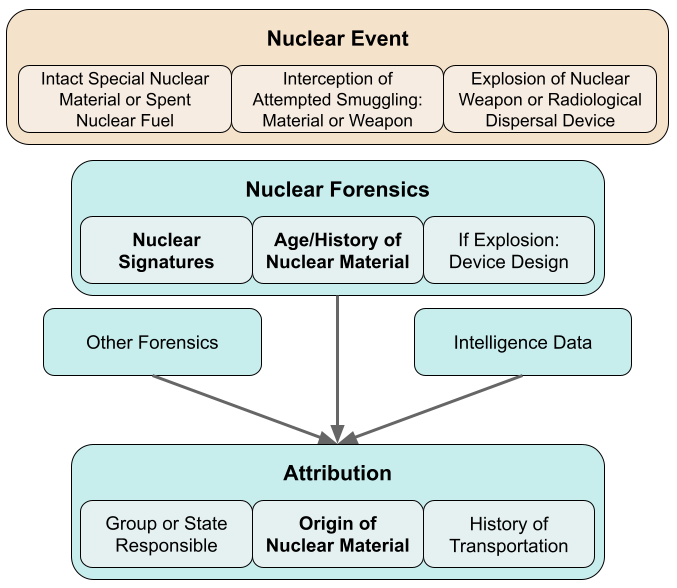
\includegraphics[height=0.85\textheight]{./figures/nf_define.png}
  \end{figure}
\end{frame}

\begin{frame}
  \frametitle{Nuclear Forensics}
  \begin{figure}
    \centering
    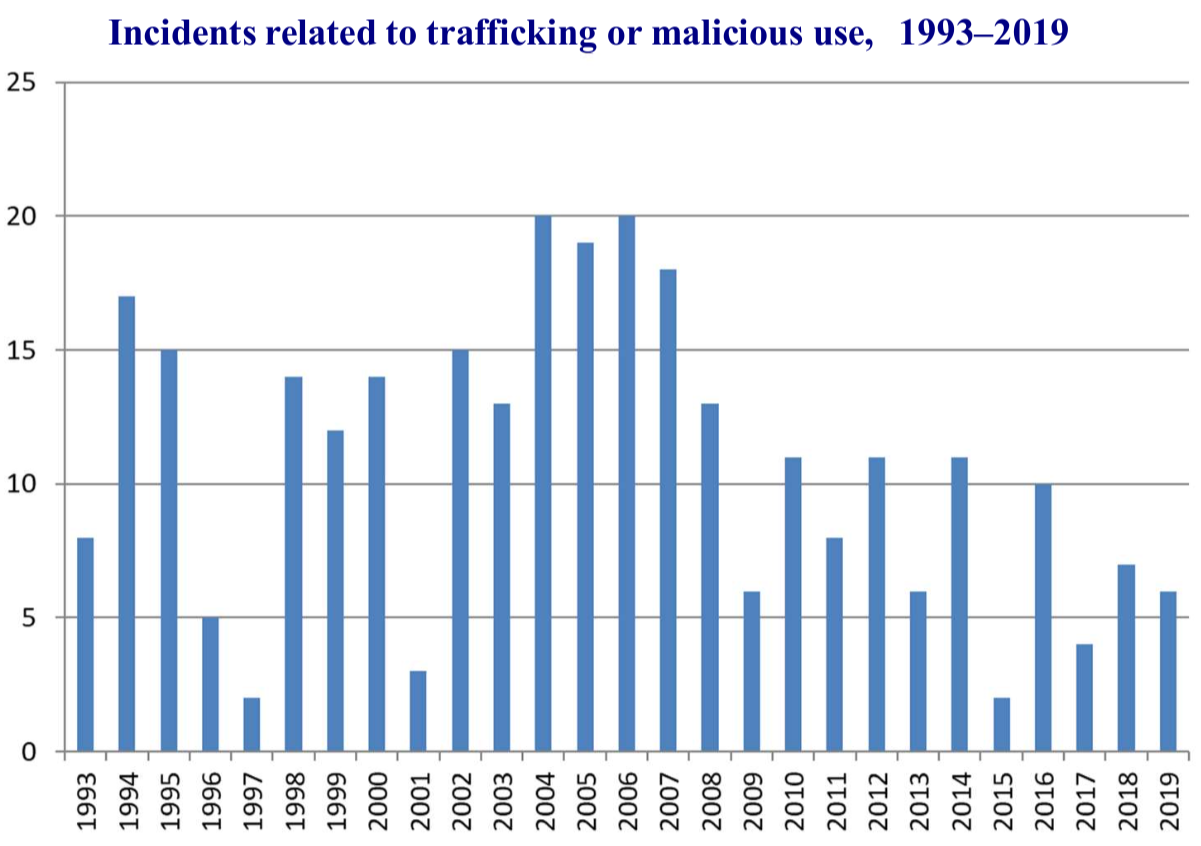
\includegraphics[width=0.78\textwidth]{./figures/nucleartrafficking.png}
  \end{figure}
  Incidents of highest concern: Highly enriched uranium (12), plutonium (2), 
  plutonium-beryllium neutron sources (5) \cite{itdb}
\end{frame}

\begin{frame}
  \frametitle{Nuclear Forensics Investigations}
  Slide on timeline of nuclear forensics investigation\\~\\
  Tradeoff of time and information
\end{frame}

\begin{frame}
  \frametitle{Main Goal}

  Is it possible to \textbf{speed up} a nuclear forensics
  \textbf{investigation} of spent nuclear fuel with \textbf{field-deployable
  detection}?

\end{frame}

\begin{frame}
  \frametitle{Statistical Methods}

  Why are statistical methods being used

\end{frame}

